
%%%%%%%%%%%%%%%%%%%%%%%%%%%%%%%%%%%%%%%%%%%%%%%%%%%%%%%%%%%%%%%%%%%%%%%
%% DOKUMENTVORLAGE THOMAS DIETRICH  %%%%%%%%%%%%%%%%%%%%%%%%%%%%%%%%%%%
%%%%%%%%%%%%%%%%%%%%%%%%%%%%%%%%%%%%%%%%%%%%%%%%%%%%%%%%%%%%%%%%%%%%%%%

\documentclass[
		12pt,						% Schriftgr��e
		ngerman,					% f�r Umlaute, Silbentrennung etc.
		a4paper,					% Papierformat
		oneside,					% einseitiges Dokument
		%twoside,					% zweiseitiges Dokument
		titlepage,					% es wird eine Titelseite verwendet
		parskip=half,				% Abstand zwischen Abs�tzen (halbe Zeile)
		headings=normal,			% Gr��e der �berschriften verkleinern
		open=right,					% Chapter beginnen rechts
		listof=totoc,				% Verzeichnisse im Inhaltsverzeichnis auff�hren
		bibliography=totoc,			% Literaturverzeichnis im Inhaltsverzeichnis auff�hren
		captions=tableheading,		% Beschriftung von Tabellen unterhalb ausgeben
		draft=true, 				% TODO: Entwurfsmodus, im finalen Dokument auf false zu setzen
]{scrreprt} 
%%%%%%%%%%%%%%%%%%%%%%%%%%%%%%%%%%%%%%%%%%%%%%%%%%%%%%%%%%%%%%%%%%%%%%%

 
%% Schrift und Deutsch %%%%%%%%%%%%%%%%%%%%%%%%%%%%%%%%%%%%%%%%%%%%%%%%
%\usepackage[ngerman]{babel}
\usepackage[T1]{fontenc}
\usepackage[ansinew]{inputenc} 
\usepackage{textcomp} % Euro-Zeichen etc.
\usepackage{lmodern}

%\usepackage[T1]{fontenc}
%\usepackage[utf8x]{inputenc}
%\usepackage{libertine}
%\usepackage[ngerman]{babel}

%\usepackage{xunicode}
%\usepackage{fontspec}
%\usepackage{xltxtra} % f�r XeLaTeX 
%\setromanfont[Mapping=tex-text]{Linux Libertine O} % Serifenschrift
%\setsansfont[Mapping=tex-text]{Linux Biolinum O} % serifenlose Schrift
%\setmonofont[Mapping=tex-text,Scale=0.9]{Courier New} % Schriftart f�r Code
%\setmonofont[Mapping=tex-text]{DejaVu Sans Mono}
%\usepackage{polyglossia}
%\setdefaultlanguage[spelling=new,latesthyphen=true]{german} 

 
%%%%%%%%%%%%%%%%%%%%%%%%%%%%%%%%%%%%%%%%%%%%%%%%%%%%%%%%%%%%%%%%%%%%%%%

 
%% Globale Dokument-Informationen %%%%%%%%%%%%%%%%%%%%%%%%%%%%%%%%%%%%%
\newcommand{\arbeitstitel}{How To Write A Research Document}
\newcommand{\arbeitstitelexample}{Your title here}
\newcommand{\arbeitsart}{Research Seminar}
\newcommand{\autor}{Your name}
\newcommand{\mail}{Your email ID}
\newcommand{\studiengang}{Ingenieurinformatik}
\newcommand{\matrikelnr}{012345}
\newcommand{\erstgutachter}{Prof. Dr.-Ing. habil. Armin Zimmermann}
\newcommand{\zweitgutachter}{M.Sc. Thomas Dietrich}
\newcommand{\fakultaet}{Faculty of Computer Science and Automation}
\newcommand{\fachgebiet}{System and Software Engineering}
\newcommand{\ort}{Ilmenau}
\newcommand{\ausgabedatum}{Your start date}
\newcommand{\abgabedatum}{Your end date}
\newcommand{\version}{v1.0 2015-01-04}
%%%%%%%%%%%%%%%%%%%%%%%%%%%%%%%%%%%%%%%%%%%%%%%%%%%%%%%%%%%%%%%%%%%%%%%


%% Packages f�r Grafiken & Abbildungen %%%%%%%%%%%%%%%%%%%%%%%%%%%%%%%%
\usepackage{graphicx}			% Zum Laden von Grafiken
\usepackage{wrapfig}			% Einbinden von Grafiken mit umflie�endem Text
\usepackage{subfig}				% Einbinden von mehreren Objekten innerhalb eines floats
\usepackage{pdfpages}			% bindet eine Grafikdatei (.pdf oder .jpg) seitenf�llend in das Dokument ein
\graphicspath{{Bilder/}}
\usepackage[normalem]{ulem}
%%%%%%%%%%%%%%%%%%%%%%%%%%%%%%%%%%%%%%%%%%%%%%%%%%%%%%%%%%%%%%%%%%%%%%%


%% Zeilenabst�nde und Seitenr�nde %%%%%%%%%%%%%%%%%%%%%%%%%%%%%%%%%%%%%
\usepackage{setspace}
\usepackage{geometry}
%%%%%%%%%%%%%%%%%%%%%%%%%%%%%%%%%%%%%%%%%%%%%%%%%%%%%%%%%%%%%%%%%%%%%%%


%% Literaturverzeichnis %%%%%%%%%%%%%%%%%%%%%%%%%%%%%%%%%%%%%%%%%%%%%%%
\usepackage[numbers,square]{natbib}
\bibliographystyle{alphadin}
%%%%%%%%%%%%%%%%%%%%%%%%%%%%%%%%%%%%%%%%%%%%%%%%%%%%%%%%%%%%%%%%%%%%%%%


%% TODOs %%%%%%%%%%%%%%%%%%%%%%%%%%%%%%%%%%%%%%%%%%%%%%%%%%%%%%%%%%%%%%
%\usepackage{pdfcomment}

\usepackage[%
		%disable,				% deaktiviert das Package
		german,
		textsize=tiny,
		colorinlistoftodos
]{todonotes}
\newcommand{\todoref}[1]{\todo[color=blue!40]{Missing Reference #1}}
\newcommand{\todoedit}[1]{\todo[color=green!40]{#1}}
%%%%%%%%%%%%%%%%%%%%%%%%%%%%%%%%%%%%%%%%%%%%%%%%%%%%%%%%%%%%%%%%%%%%%%% 


%% HyperRef %%%%%%%%%%%%%%%%%%%%%%%%%%%%%%%%%%%%%%%%%%%%%%%%%%%%%%%%%%%
% http://www.tug.org/applications/hyperref/manual.html
\usepackage{hyperref}
\hypersetup{
		pdftitle={\arbeitstitel},	% Sets the document information Title field
		pdfauthor={\autor},			% Sets the document information Author field
		pdfsubject={\arbeitsart},	% Sets the document information Subject field
		%backref=section,			% adds backlink text to the end of each item in the bibliography, as a list of section numbers
		%pdfpagelabels,
		pdfpagelayout=TwoColumnRight, 
		%pdfpagelayout=TwoPageRight, % Displays two pages, odd-numbered pages to the right % Achtung, PDF-Version 1.5 erforderlich
		%pdfdisplaydoctitle=true,	% display document title instead of file name in title bar
		hypertexnames=false,		% zur korrekten Erstellung der Bookmarks
		%linktocpage 				% Seitenzahlen anstatt Text im Inhaltsverzeichnis verlinken
		%bookmarks, 
		bookmarksnumbered=true,
		bookmarksopen=true,  
		bookmarksopenlevel=1,
		%hyperfootnotes=true, 
		%unicode=true, 
		colorlinks=true, 
% diese Farbdefinitionen sollten f�r den Druck verwendet werden (alles schwarz)
%		linkcolor=black, 		% einfache interne Verkn�pfungen
%		anchorcolor=black, 		% Ankertext
%		citecolor=black, 		% Verweise auf Literaturverzeichniseintr�ge im Text
%		filecolor=black, 		% Verkn�pfungen, die lokale Dateien �ffnen
%		menucolor=black, 		% Acrobat-Men�punkte
%		urlcolor=black, 		% Farbe des verlinkten Textes externe URLs
% diese Farbdefinitionen kann f�r farbigen Druck oder f�r die weitergabe als PDF verwendet werden
		linkcolor=darkblue,		% einfache interne Verkn�pfungen
		citecolor=darkblue, 	% Verweise auf Literaturverzeichniseintr�ge im Text
		menucolor=darkblue,		% Acrobat-Men�punkte
		urlcolor=cyan, 			% Farbe des verlinkten Textes externe URLs
}

% URL verlinken, lange URLs umbrechen etc.
\usepackage{url}
%%%%%%%%%%%%%%%%%%%%%%%%%%%%%%%%%%%%%%%%%%%%%%%%%%%%%%%%%%%%%%%%%%%%%%%

  
%% Absatzeinstellung %%%%%%%%%%%%%%%%%%%%%%%%%%%%%%%%%%%%%%%%%%%%%%%%%%
%\setlength{\parskip}{3pt}
%\setlength{\parindent}{0pt}
%%%%%%%%%%%%%%%%%%%%%%%%%%%%%%%%%%%%%%%%%%%%%%%%%%%%%%%%%%%%%%%%%%%%%%%


%% Abk�rzungsverzeichnis %%%%%%%%%%%%%%%%%%%%%%%%%%%%%%%%%%%%%%%%%%%%%%
\usepackage[intoc]{nomencl}
\let\abbrev\nomenclature
% Deutsche �berschrift
\renewcommand{\nomname}{Abk�rzungsverzeichnis}
% Punkte zw. Abk�rzung und Erkl�rung
\setlength{\nomlabelwidth}{.25\hsize}
\renewcommand{\nomlabel}[1]{#1 \dotfill}
% Zeilenabst�nde verkleinern
\setlength{\nomitemsep}{-\parsep}
%%%%%%%%%%%%%%%%%%%%%%%%%%%%%%%%%%%%%%%%%%%%%%%%%%%%%%%%%%%%%%%%%%%%%%%

%%%%%%%%%%%%%%%%%%%%%%%%%%%%%%%%%%%%%%%%%%%%%%%%%%%%%%%%%%%%%%%%%%%%%%%
\usepackage{siunitx}
% Nutzung:
%   \SI[options]{value}[pre-unit]{unit}
%   \si[options]{unit}
%   \num[options]{number}
%   \ang[options]{angle}
\sisetup{
	locale=DE,
	load-configurations=binary,
	load-configurations=abbreviations,
	per-mode=symbol,
}
\DeclareSIUnit\bit{Bit}
\DeclareSIUnit\byte{Byte}
%%%%%%%%%%%%%%%%%%%%%%%%%%%%%%%%%%%%%%%%%%%%%%%%%%%%%%%%%%%%%%%%%%%%%%%

%%%%%%%%%%%%%%%%%%%%%%%%%%%%%%%%%%%%%%%%%%%%%%%%%%%%%%%%%%%%%%%%%%%%%%%
\usepackage{booktabs}
\setlength{\belowbottomsep}{\belowrulesep} %Ersetzt 0pt-Abstand zwischen bottomrule und Caption
% Nutzung:
%   \toprule, \midrule, \bottomrule
%   \cmidrule, \addlinespace
%%%%%%%%%%%%%%%%%%%%%%%%%%%%%%%%%%%%%%%%%%%%%%%%%%%%%%%%%%%%%%%%%%%%%%%

%% Verschiedenes %%%%%%%%%%%%%%%%%%%%%%%%%%%%%%%%%%%%%%%%%%%%%%%%%%%%%%
\usepackage{ifdraft}					% In Abh�ngigkeit von draft bzw. final Aktionen ausf�hren % \ifdraft{draft case}{final case}
\usepackage{pdfpages} 					% pdf import
\usepackage{amsmath,amssymb,amstext} 	% f�r mathematische Symbole
\usepackage{upgreek}					% f�r nicht-kursive griechische Buchstaben, Bsp. \uppi
%\usepackage{array}
\usepackage{xspace}
\usepackage{xcolor}
\usepackage{multirow}
\usepackage{listings} 					% Programmcode
%\usepackage{chngcntr} 					% fortlaufendes Durchnummerieren der Fu�noten
\usepackage[perpage]{footmisc}
% Kopf- und Fu�zeilen anpassen
\usepackage[
		automark, 						% Kapitelangaben in Kopfzeile automatisch erstellen
		headsepline, 					% Trennlinie unter Kopfzeile
%		footsepline, 					% Trennlinie �ber Fu�zeile
		ilines 							% Trennlinie linksb�ndig ausrichten
]{scrpage2}
  
\usepackage{caption} 
\captionsetup{format=hang,margin=30pt,font=small,labelfont=bf,labelsep=endash}

\usepackage{paralist}

\usepackage[yyyymmdd,hhmmss]{datetime}
%%%%%%%%%%%%%%%%%%%%%%%%%%%%%%%%%%%%%%%%%%%%%%%%%%%%%%%%%%%%%%%%%%%%%%%
 

%%%%%%%%%%%%%%%%%%%%%%%%%%%%%%%%%%%%%%%%%%%%%%%%%%%%%%%%%%%%%%%%%%%%%%%
%%%%%%%%%%%%%%%%%%%%%%%%%%%%%%%%%%%%%%%%%%%%%%%%%%%%%%%%%%%%%%%%%%%%%%%

\makenomenclature

%% Seitenstil %%%%%%%%%%%%%%%%%%%%%%%%%%%%%%%%%%%%%%%%%%%%%%%%%%%%%%%%%
% Zeilenabstand 1,5
\onehalfspacing 
%\linespread{1.5}

\setlength{\topskip}{\ht\strutbox} % behebt Warnung von geometry
\geometry{paper=a4paper,left=30mm,right=18mm,top=15mm,bottom=55mm}

\pagestyle{scrheadings} % Kopf- und Fu�zeilen
\renewcommand*{\chapterpagestyle}{scrheadings} % Kopf- und Fu�zeile auch auf Kapitelanfangsseiten 
\renewcommand{\headfont}{\normalfont} % Schriftform der Kopfzeile

%TODO: fancyhdr

% Kopfzeile
%\ihead{\large{\textsc{\arbeitstitel}}\\ \small{\arbeitstitel} \\[2ex] \textit{\headmark}}
%\ihead{\large{\textsc{\arbeitsart}}\ - \small{\autor} \\ \textit{\headmark}}
\ihead{\textit{\headmark}}
\chead{}
\ohead{\pagemark}
%\ohead{\includegraphics[scale=0.15]{\logo}}
\setlength{\headheight}{30mm} % H�he der Kopfzeile
% Kopfzeile �ber den Text hinaus verbreitern
\setheadwidth[0pt]{textwithmarginpar} 
\setheadsepline[text]{0.4pt} % Trennlinie unter Kopfzeile

% Fu�zeile
%\ifoot{\small{\arbeitsart\ \autor}}
\ifoot{}
\cfoot{}
\ofoot{\pagemark}

%% Verschiedenes %%%%%%%%%%%%%%%%%%%%%%%%%%%%%%%%%%%%%%%%%%%%%%%%%%%%%%
\frenchspacing % erzeugt ein wenig mehr Platz hinter einem Punkt

% Hurenkind und Schusterjunge vermeiden (http://de.wikipedia.org/wiki/Hurenkind)
\clubpenalty = 10000
\widowpenalty = 10000
\displaywidowpenalty = 10000

% Fu�noten fortlaufend durchnummerieren
%\counterwithout{footnote}{chapter}

% Farben f�r Listings
\definecolor{darkblue}{rgb}{0,0,.5}
\definecolor{hellgelb}{rgb}{1,1,0.9}
\definecolor{hellgrau}{rgb}{0.95,0.95,0.95}
\definecolor{colKeys}{rgb}{0,0,1}
\definecolor{colIdentifier}{rgb}{0,0,0}
%\definecolor{colComments}{rgb}{1,0,0}		%rot
%\definecolor{colComments}{rgb}{0.1,0.5,0}	%gr�n
\definecolor{colComments}{rgb}{0.5,0.5,0.5}	%grau
\definecolor{colString}{rgb}{0,0.5,0}

% Quellcode-Ausgabe formatieren
\renewcommand{\lstlistlistingname}{Verzeichnis der Quelltexte} 
\renewcommand{\lstlistingname}{Quelltext}
\lstset{
		float=tbph,												% makes sense on individual displayed listings only and lets them float
		language=C++,											% choose the language of the code
		basicstyle=\footnotesize,								% the size of the fonts that are used for the code
		numbers=left,											% where to put the line-numbers
		numberstyle=\tiny,										% the size of the fonts that are used for the line-numbers
		%numberstyle=\footnotesize,								% the size of the fonts that are used for the line-numbers
		stepnumber=1,											% the step between two line-numbers. If it's 1 each line will be numbered
		numbersep=7pt,											% how far the line-numbers are from the code
		backgroundcolor=\color{hellgelb},						% choose the background color. You must add \usepackage{color}
		showspaces=false,										% show spaces adding particular underscores
		showstringspaces=false,									% underline spaces within strings
		showtabs=false,											% show tabs within strings adding particular underscores
		frame=single,											% adds a frame around the code
%		frame={trLb},											% adds a frame around the code
		tabsize=4,												% sets default tabsize to 2 spaces
		captionpos=b,											% sets the caption-position (b or t)
		breaklines=true,										% sets automatic line breaking
		breakatwhitespace=false,								% sets if automatic breaks should only happen at whitespace
		breakindent=5pt,										% is the indention of the second, third,... line of broken lines
%		escapeinside={\%*}{*)},									% if you want to add a comment within your code
		identifierstyle=\color{colIdentifier},
		keywordstyle=\color{colKeys},
		stringstyle=\color{colString},
		commentstyle=\color{colComments},
		columns=fixed,
		%emph={bool,int,unsigned,char,true,false,void}, emphstyle=\color{blue},
		%emph={[2]\#include,\#define,\#ifdef,\#endif}, emphstyle={[2]\color{darkblue}},
}

% Neuberechnung des Satzspiegels (zur Vermeidung von overfull boxes)
%\KOMAoptions{DIV=last}

%%%%%%%%%%%%%%%%%%%%%%%%%%%%%%%%%%%%%%%%%%%%%%%%%%%%%%%%%%%%%%%%%%%%%%%
%%%%%%%%%%%%%%%%%%%%%%%%%%%%%%%%%%%%%%%%%%%%%%%%%%%%%%%%%%%%%%%%%%%%%%%

%% Befehle %%%%%%%%%%%%%%%%%%%%%%%%%%%%%%%%%%%%%%%%%%%%%%%%%%%%%%%%%%%%
 
% Abk�rzungen mit korrektem Leerraum 
%\newcommand{\ua}{\mbox{u.\,a.\ }}
%\newcommand{\zB}{\mbox{z.\,B.\ }}
%\newcommand{\dahe}{\mbox{d.\,h.\ }}
\newcommand{\iic}{\mbox{I\texttwosuperior C}} % I�C
%\newcommand{\iic}{\mbox{I�C}} % I�C

%%%%%%%%%%%%%%%%%%%%%%%%%%%%%%%%%%%%%%%%%%%%%%%%%%%%%%%%%%%%%%%%%%%%%%%
%% DOKUMENTVORLAGE THOMAS DIETRICH  %%%%%%%%%%%%%%%%%%%%%%%%%%%%%%%%%%%
%%%%%%%%%%%%%%%%%%%%%%%%%%%%%%%%%%%%%%%%%%%%%%%%%%%%%%%%%%%%%%%%%%%%%%%


%%%%%%%%%%%%%%%%%%%%%%%%%%%%%%%%%%%%%%%%%%%%%%%%%%%%%%%%%%%%%%%%%%%%%%%
%% DOKUMENTVORLAGE THOMAS DIETRICH  %%%%%%%%%%%%%%%%%%%%%%%%%%%%%%%%%%%
%%%%%%%%%%%%%%%%%%%%%%%%%%%%%%%%%%%%%%%%%%%%%%%%%%%%%%%%%%%%%%%%%%%%%%%

\begin{document}
%%%%%%%%%%%%%%%%%%%%%%%%%%%%%%%%%%%%%%%%%%%%%%%%%%%%%%%%%%%%%%%%%%%%%%%
%% Titelseite und folgendes
%%%%%%%%%%%%%%%%%%%%%%%%%%%%%%%%%%%%%%%%%%%%%%%%%%%%%%%%%%%%%%%%%%%%%%%
\pdfbookmark{\arbeitsart{} \autor}{\arbeitsart{} \autor}
\begin{titlepage}
\thispagestyle{empty}

\begin{center} 
	
\includegraphics[scale=1]{Logo_schwarzgruen_RGB_04.jpg}\\[0ex]
	%Technische Universit�t Ilmenau\\[0ex]
	\fakultaet\\[0ex]
	\fachgebiet\\[8ex]
	%\Huge{\textbf{\arbeitsart}}\\[0ex]
	\Large{\textbf{\arbeitstitel}}\\[1.5ex]
	
	\vfill 
	
	\normalsize
	\begin{tabular}{lll}
		%\textbf{Start Date:}					& & \ausgabedatum				\\[0.5ex]
		%\textbf{End Date:}					& & \abgabedatum				\\[0.5ex]
												%& & 							\\[0.5ex]
		\textbf{Responsible Professor:}	& & \erstgutachter				\\[0.5ex]
		\textbf{Advisor:}	& & \zweitgutachter				\\[0.5ex]
												& & 							\\[0.5ex]
												\version
		%\textbf{Submitted by:} 				& & \autor						\\[0.5ex]
											%	& & Matrikel-Nr. \matrikelnr	\\[0.5ex]
											%	& & \mail						\\[0.5ex]
	\end{tabular}
\end{center}  

%TODO: draft
%\raggedleft \tiny \ifdraft{draft version, compiled on \today\ at \currenttime}{finale Version}

\end{titlepage}
\chapter*{Change History}
\thispagestyle{empty}
\begin{table}[h]
\begin{tabular}{lll}
\toprule
v1.0 2015-01-04 & Samrudhi Shingavi & Initial version of the document \\
\midrule
\end{tabular}
\end{table}
\begin{titlepage}
\thispagestyle{empty}

\begin{center} 
	
\includegraphics[scale=1]{Logo_schwarzgruen_RGB_04.jpg}\\[0ex]
	%Technische Universit�t Ilmenau\\[0ex]
	\fakultaet\\[0ex]
	\fachgebiet\\[8ex]
	%\Huge{\textbf{\arbeitsart}}\\[0ex]
	\Large{\textbf{\arbeitstitelexample}}\\[1.5ex]
	
	\vfill 
	
	\normalsize
	\begin{tabular}{lll}
		\textbf{Start Date:}					& & \ausgabedatum				\\[0.5ex]
		\textbf{End Date:}					& & \abgabedatum				\\[0.5ex]
												& & 							\\[0.5ex]
		\textbf{Responsible Professor:}	& & \erstgutachter				\\[0.5ex]
		\textbf{Advisor:}	& & \zweitgutachter				\\[0.5ex]
												& & 							\\[0.5ex]
		\textbf{Submitted by:} 				& & \autor						\\[0.5ex]
												& & Matriculation-Nr. \matrikelnr	\\[0.5ex]
												& & \mail						\\[0.5ex]
	\end{tabular}
\end{center}  

%TODO: draft
%\raggedleft \tiny \ifdraft{draft version, compiled on \today\ at \currenttime}{finale Version}

\end{titlepage}
%\chapter*{Thanks}
\thispagestyle{empty}

\begin{quote}
An dieser Stelle m�chte ich \ldots
\end{quote} 

\cleardoublepage{}   
\pdfbookmark{Abstract}{Abstract}   
\chapter*{Abstract}
\thispagestyle{empty}
An abstract comprises a one-paragraph summary of the whole paper.
Abstracts have become increasingly important, as electronic publication databases
are the primary means of finding research reports in a certain subject area
today \cite{Koopman1997}.

According to \cite{Day2012}, there are two basic types of abstract:
\begin{itemize}
  \item An \textit{informative} abstract extracts everything relevant from the
  paper, such as research objectives addressed, methods employed in solving the problems,
results obtained, and conclusions drawn. Such abstracts may serve as a highly
aggregated substitute for the full paper.
\item An \textit{indicative or descriptive} abstract rather describes the
content of the paper and may thus serve as an outline of what is presented in
the paper. This kind of abstract cannot serve as a substitute for the full text.
\end{itemize}
A checklist defining relevant parts of an abstract is proposed in
\cite{Koopman1997}:
\begin{itemize}
\item \uline{Motivation:} Why do we care about the problem and the results?
\item \uline{Problem:} What problem is the paper trying to solve and what is
the scope of the work?
\item \uline{Solution:} What was done to solve the problem?
\item \uline{Results:} What is the answer to the problem?
\item \uline{Conclusions:} What conclusions does the answer imply?
\end{itemize}
Also as suggested in \cite{Day2012} there are few things that should not be
included in an abstract, i.e. information and conclusions not stated in the
paper, the exact title phrase, and illustrative elements such as tables and figures.  It is also
not beneficial to use the exact phrases that appear later in the introduction.  


\nomenclature{UART}{Universal Asynchronous Receiver Transmitter}
%\nomenclature{}{}
%\nomenclature{}{}
%\nomenclature{}{}
%\nomenclature{}{}	% nur Definitionen, kein sichtbarer Dokumentinhalt
% f�r weitere Informationen siehe <http://de.wikibooks.org/wiki/LaTeX-W%C3%B6rterbuch:_Silbentrennung>
\hyphenation{}	% nur Definitionen, kein sichtbarer Dokumentinhalt
\cleardoublepage{}

\pagenumbering{roman}
\pdfbookmark{Inhaltsverzeichnis}{Inhaltsverzeichnis}
\tableofcontents
\cleardoublepage{}

%%%%%%%%%%%%%%%%%%%%%%%%%%%%%%%%%%%%%%%%%%%%%%%%%%%%%%%%%%%%%%%%%%%%%%%
%% Hauptteil
%%%%%%%%%%%%%%%%%%%%%%%%%%%%%%%%%%%%%%%%%%%%%%%%%%%%%%%%%%%%%%%%%%%%%%%
\pagenumbering{arabic} 
%%%%%%%%%%%%%%%%%%%%%%%%%%%%%%%%%%%%%%%%%%%%%%%%%%%%%%%%%%%%%%%%%%%%%%%
%% 
%%%%%%%%%%%%%%%%%%%%%%%%%%%%%%%%%%%%%%%%%%%%%%%%%%%%%%%%%%%%%%%%%%%%%%%
\chapter{Introduction}

In the Introduction, you are attempting to inform the reader about the rationale
behind the work, justifying why your work is an essential component of research
in the field. The introduction gives an overall review of the paper. Much  of 
the Introduction  should  be  written  in  the  present  tense, because  the  problem  and  the established  knowledge relating  to  it  at  the  start
of  the  work will  be primarily referred.

As recommended in \cite{Majid1993}, the Introduction should be structured as
follows:

 \uline {Motivation and Background Information.}
 This should recall to the reader why the kind of result mentioned already in
 the abstract would be interesting and important. 
 It states the motivation, so if the reader agrees with the way you are
 looking at the field, there's some probability that the paper will be useful
 for them. Also purpose in writing the paper should be clearly stated.
 Sufficient  background  information should be supplied to  allow the  reader  
to understand  and  evaluate the  results  of  the  present study.
\par  \uline{The results and strategy.}
 It should present first, the nature and scope of the  problem  investigated.
 It should state the method and principal results of the investigation
 \cite{Day2012}. Reference the previous work which inspired and led up to your
 result. A good way is to tell a story, an interesting one that puts everything
 into perspective are the existing literature and conveys how it is you succeeded where others
failed. What was the key idea which nobody else spotted? The reader should not
be kept in suspense; instead allowed to follow the development of the evidence.
 
\par \uline{Outline the organisation.}
This should be brief but not simply a list. State the goal and main achievement
of each section. Make it into a story whereby each section is logically a
precursor to the next section. 

The aim of this report is to guide in creating a plan that motivates original thinking and
 to only do your own best. It also provides information on how to work on
 a research document. It covers the entire process which includes
 gathering requirements, searching for information about the topic,
 proposing working answers and supporting them and writing the research
 document.


%%%%%%%%%%%%%%%%%%%%%%%%%%%%%%%%%%%%%%%%%%%%%%%%%%%%%%%%%%%%%%%%%%%%%%%
%% 
%%%%%%%%%%%%%%%%%%%%%%%%%%%%%%%%%%%%%%%%%%%%%%%%%%%%%%%%%%%%%%%%%%%%%%%
\chapter{Research Process}
Research is the persevering, thorough study into a subject that requires time
and effort on your part. The research process is a step-by-step process of developing a research paper.
It is a multiple-step process where the steps are interlinked with the other
steps in the process.
 
\begin{figure}[htb]
\begin{center} 
  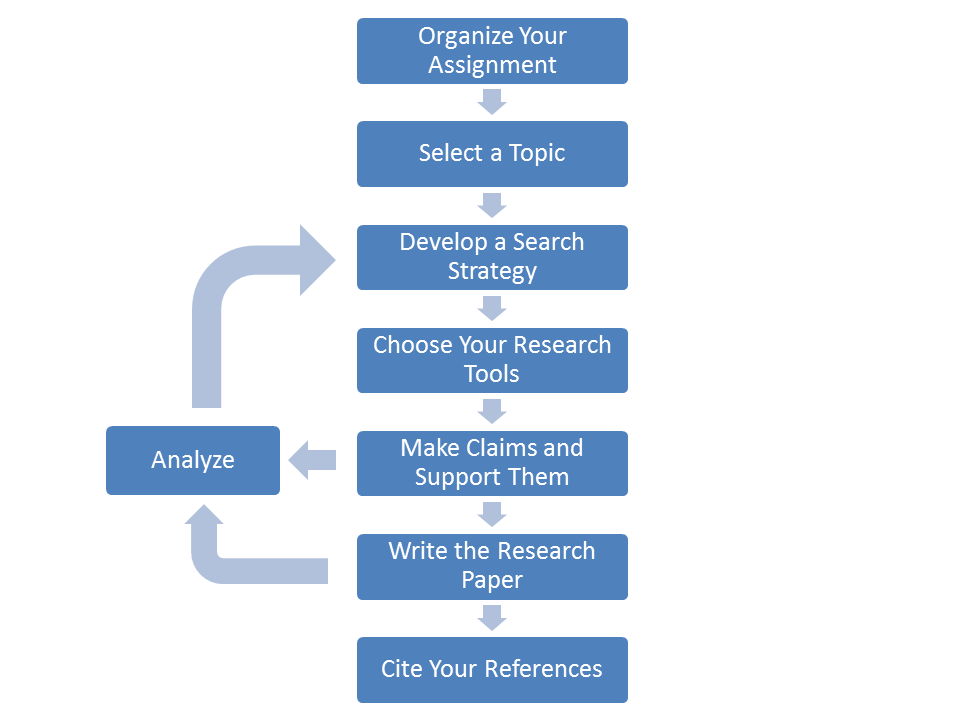
\includegraphics[width=0.60\textwidth]{ResearchProcess_steps}  
  \caption{Research Process}
  \label{fig:Research Process}
\end{center}
\end{figure}
Figure 2.1 is a graphical representation of the steps involved in the research
process. The first four steps are a part of the the Planning process. Further
three steps represents different stages of creation of a scientific report.
Also, you may need to go back and repeat some of these steps.These steps are
elaborated further in this report.
\section{Objectives Of Research Process} 
\label{sec:objectives} 
The aim of doing research and writing the research paper is to develop
abilities of scientific research in the students, to encourage their creativity
and promote their ideas and skills \cite{Sardiko2004}.
According to \cite{Sardiko2004} the objectives are to develop the following skills:  
\begin{itemize}
\item orientation in the literature on the subject
\item logical organization of ideas
\item in-depth study of a selected topic
\item formulation of arguments
\item planning and implementation of a research experimental part
\item data gathering, processing and analyzing
\item deriving conclusions.
\end{itemize}

\section{Questions that Researchers Ask} 
According to \cite{Turabian2007}, experienced researchers know that they are
expected to ask and answer different kinds of questions. The three kinds of
questions suggested in \cite{Turabian2007} are discussed below:
\begin{itemize}
  \item \uline{Conceptual Questions: What Should We Think?}
  A question is conceptual when the answer to So what? helps understand some
  issue but doesn't tell what is to be done:
  
  \textit{I am working on the topic X, because I want to find out
  why/how/whether Y , if I do that I can help others understand why/how/whether
  Z}
  
  \item \uline{Practical Questions: What Should We Do?}
  A question is conceptual when the answer to So what? tells what is to be done
  to change or fix some situation:
  
  \textit{I am working on the topic X, because I want to find out
   Y , if I do that I can tell others what to do to fix/improve Z}
   
   \item \uline{Applied Questions: What Must We Understand before We Know What
   To Do?} 
   Often research needs to be done in order to understand the problem better.
   This kind of research is called \textit{applied} research. The solution to
   this problem is not a solution to the practical problem but a step towards
   it.
\end{itemize}
\chapter{Planning}
\label{sec:planning}
\section{Organize Your Assignment} 
\label{sec:planning:sizeup}
The first step in the research process is to examine your assignment to determine 
what the professor is looking for and what guidelines has been given to you for
the assignment.
In \cite{au2012}, it is suggested to take note of the following:
\begin{itemize}
\item \uline{Topic:} Has the professor assigned a specific topic
or topics for you to write about, or can you choose a subject of interest to you within the 
scope of the course? 
\item  \uline {Type of research:} Does the assignment require original
research or does it require secondary research (the interpretation of previously published research 
found in books or journal articles)? 
\item  \uline{Scope:} Does the professor want you to analyse a topic from
different viewpoints, or do you need to take one position and defend it? 
\item  \uline{Sources:} Are you required to use a certain number and/or type
of sources in your research? 
\item  \uline{Length:} Has the professor set a page or word limit on the paper? 
\item  \uline{Format:} Has the professor given any guidelines regarding the
layout of the paper, such as line spacing or use of page numbers? 
\item  \uline{Citation style:} Has the professor specified a citation style
for you to use in citing your sources? If not, which style is appropriate for your subject?
\item  \uline{Due date:} When is your paper due? Do you have enough time to
 obtain all the materials you will need?
\end{itemize}
\section{Develop a Search Strategy} 
\label{sec:planning:searchStrategy}
As stated in \cite{au2012}, a search strategy is what you use to search for
information in the journal databases, on the web, and in Library catalogues. Formulating a search strategy requires you to analyze your research 
question in order to isolate the major concepts, and then develop a search query based on those
concepts. In other words, you will determine what search terms you want to search for and then
plan how you will search for that information.

\section{Choose Your Research Tools}
\label{sec:planning:researchTools}
Once the research topic is selected, reliable sources can be looked at to find
relevant information regarding the topic. In \cite{Turabian2007} it is recommended
that the sources are reliable if they satisfy at least one of these
characteristics:
\begin{itemize}
\item The source is published by a reputable press
\item The publisher uses peer reviews for everything it publishes
\item The author is a reputable scholar
\item The source is current
\item The sources has received good reviews
\item The source has been frequently cited by others
\end{itemize}
\subsection{Kinds of Sources}
According to \cite{Turabian2007}, there are three levels of sources, called
\textit{primary, secondary} and \textit{tertiary}.  As stated in
\cite{Turabian2007}, the description of these sources is as follows:
\begin{itemize}
  \item \uline{Read Primary Sources for Evidence.}
 Data is collected by researchers through observation and experiment. The
 evidence consists of this collected data. The publications that publish these
 collected data are the primary sources for them. The publications can be can
 range from government and commercial databases to scholarly jornals. Primary
 sources should be looked upon first for searching the data.
 \item  \uline{Read Secondary Sources to Learn.}
 Secondary sources are books and articles that analyze primary sources. They
 also include specialized encyclopedias and dictionaries that offer essays written by
 other scholars in a field. Secondary sources are normally used to keep up with
 the current work by informing and refining its thinking , motivating its
 work and making an contibution to a published line of research. They are also
 used to \textit{find others points of view} and \textit{find models for your
 own research and analysis}
 
 Data should be used from secondary resources when it couldn't be found in
 primary sources. You have to be cautious about using it as it can have high
 error rate. These sources may assume a lot of background knowledge. In this
 case, you can refer to tertiary sources.
 
 \item  \uline{Read Tertiary Sources for Introductory Reviews.}
 Tertiary sources are based on secondary sources and written for
 non-specialists. They include general encyclopedias and dictionaries,
 newspapers and commercial books. Well edited encyclopedias offer quick
 overview of many topics .Howerver, online encyclopedias like Wikipedia rely on
 anonymous information so it should never be cited as authoritive source.
\end{itemize}

\subsection{Search for Sources}
Once you understand kinds of sources, you can start looking for them.
 As stated in \cite{Turabian2007}, it is possible to find the data from the following
 sources:
\begin{itemize}
  \item \uline{Internet:} Some preliminary work can be done using a
  scholarly search engine such as Google Scholar. It will provide a rough idea
  of the kinds of sources available.
   \item \uline{Reference Librarians:} If you don't know how to find
   what you need, ask a librarian. Most college libraries offer tours of
   reference rooms and seminar on searching for information.
    \item \uline{Reference Area:} Browse the shelves in your library's reference
    room that hold the guides to your field's particular research methods,
    databases and special resources. Atleast familiarize yourself with
    bibligraphy of works published each year in your field, summary
    bibliographies of works on a specific topic collected over years,
    reviews of year work by searching for a title in your field beginning
    with 'Reviews in', Web sites maintained by individual or scholarly
    associations in case the field is new.
	\item \uline{Specialized Reference Works:} Look up your topic in specialized
	encyclopedias where you may find an overview of the topic and often a list
	of standard primary and secondary sources.
	\item \uline{Library catalog:}
	As soon as you find one
	recent book relevant to your topic, look it up in your library� s online catalog to find its
	\textit{subject headings}; they will be at the bottom of the entry.
	You can click on the subject headings to find other books on the same topics.  Many of
	those sources will have still more subject headings that can lead you to still
	more sources.

  Also search your online catalog using \textit{keywords} from your
 question or working hypothesis. If you find too many titles, start with those published 
 in the last ten years by well-known university presses.
 
If most sources on your topic are \textit{articles}, 
locate a recent one in your library� s online databases.  Its database entry will include a list 
of  keywords.  Search for them to find more articles on your topic. Some databases also 
provide abstracts of journal articles that you can skim for search terms.
\item \uline{Guides to Periodical Literature:}
The annual guides cites sources such as magazines and newspapers. 
Most specialized fields also have yearly guides to secondary
sources. 
\item \uline{Library Shelves:} 
If you work only online you may miss crucial sources that you would find only
in the library.  More important,  you will miss the benefits of an encounter
with a source that you find only in person.
Skim table of contents of the book, then its index for keywords related to
your question or its answer.  Then skim its bibliography for titles that look relevant to your project.  You can
do all that faster with books on a shelf than you can online.
\end{itemize}

As recommended in \cite{Booth2003}, at every stage of research,
\textit{guidance from the teachers} is of great help.
At first, teachers will help to focus on the question and find sources. Here, too,
the quality of the help depends on the quality of the questions one asks. The more one prepares 
before the talk with the teachers, the better it can be explained what is being done and more help 
can be received. 

\section{Planning An Outline} 
\label{sec:planning:outline}
According to \cite{Turabian2007}, some fields specify the plan of  a report. 
Readers in the experimental sciences,  for example,  expect reports to follow some version of this:
Introduction, Methods and Material, Results, Discussion, Conclusion. If you must
follow a preset plan, ask your instructor or find a secondary source for a model.  
But if you must create your own, it must make sense not just to you but visibly to your readers.  To create that visible form,  go back to your storyboard or outline.
In \cite{Booth2003} it is stated that time should be spent categorizing and
recategorizing the data to find a point of view that best reflects the thinking behind the report. 
Following steps can help to organize the report:
\begin{itemize}
\item \uline{Converting a Storyboard into an Outline}
As stated in \cite{Turabian2007}, if  you prefer to work from an outline,  you
can turn your storyboard into one.
Start with a sentence numbered I that states your claim. Add complete sentences
under it numbered II,  III and so on,  each of  which states a reason
supporting your claim.
Under each reason, use capital letters to list sentences summarizing your evidence;
then list by numbers the evidence itself. 
\item \uline{Plan a Working Introduction:}
As stated in \cite{Booth2003}, Working Introduction is enough to start on track.
It is better to create a brief context, then the research goal and its importance can be stated , followed by its 
solution just to set off in the right direction. Later it can be revised to state a 
clearer and more complete idea of the problem and proposed solution.

According to \cite{Turabian2007}, when readers see a claim in your introduction, 
they know where you are taking them and so can read what follows faster,  understand it
better,  and remember it longer.
If  you decide to announce your claim only in your conclusion, then you will
have to add a replacement sentence that includes the key terms that you
use throughout your report.
You can also add a �road map� at the end of the introduction,  laying out the
organization of  their report.
\item \uline{Organize the Body of Your Report:}
Sketch necessary background, definitions and conditions in short. Rearrange the
points into a system to form a logical structure. Decide the main points of the report. 
Put down headings. Try to acknowledge and respond to the most important questions and 
objections where there is a possibility of readers raising them.
\end{itemize}

\section{Plans To Avoid} 
\label{sec:planning:plans_avoid}
\begin{itemize}
  \item In \cite{Booth2003} it is recommended to avoid the following plans while
  creating the report:
\item \uline{Don�t Organize Your Report Around Your Assignment.}
Avoid mapping the paper onto the literal wording of their assignment. If the
assignment is echoed word to word at the beginning it gives an impression of lack of original ideas.
\item \uline{Don�t Just Summarize Sources.}
Avoid stitching together quotations from many different sources which reflects
little of own thinking. Some fields require survey of what others have written, but here the instructor looks for angle of the author in the summaries.
\item \uline{Don�t Structure Your Report Around the Topics of Your Data.}
It is better to arrange data into more analytical categories created by study of
the topic instead of organizing the report by considering the things being written about as topics.
\item \uline{Don�t Structure Your Report Around a Story of Your Research.}
Avoid giving an account of things found, overcoming obstacles, and then how the
solution was obtained by following a new lead.
\item \uline{Avoid Plagiarism.} 
The author plagiarizes when, intentionally or not, he uses someone else�s words
or ideas but fail to credit that person. It is the biggest pitfall.
\end{itemize}

\chapter{Making Claim And Supporting It}
"'When you know enough to start planning your research report, you should have a
tentative but clear understanding of your question and a tentative but reasonably specific answer.
You should have a list of reasons that support your claim. And evidence to
support those reasons'"\cite{Booth2003}.  You should also think about the
questions and objections which can be raised by the readers. "'It is difficult to
imagine all the questions but you must atleast anticipate at least the questions
that generate the five elements of an argument and answer them'"
\cite{Booth2003}.

As stated in \cite{Booth2003}, the elements of an argument are discussed below:
\begin{itemize}
  \item \uline{Argument:} "'In a research report, you make a claim, back it with reasons based on 
  evidence,acknowledge and respond to other views'"\cite{Booth2003}.
  \item \uline{Basing Claims On Reasons:} Claim is at the core of every
  research report. It is the answer to the research question, along with support for it. The support is at least one reason explaining why your claim should be
  accepted. According to \cite{Booth2003} "'A claim is any sentence that asserts
  something that may be true or false and so needs support. A reason is a
  sentence supporting a claim'".
  Usually a claim and a reason is connected using because.
  \item \uline{Basing Reasons On Evidence:} According to \cite{Booth2003},
  Evidence is something which can be seen, smelled, heard and touched. Evidence
  should be provided on which the reasons are based.
  \begin{center}
  Claim \textsubscript{because of} Reason \textsubscript{based on} Evidence
  \end{center}
  \item \uline{Acknowledging And Responding To Alternatives:} A responsible researcher supports a 
claim with reasons based on evidence. But sometimes a claim is not just
accepted on the basis of reasons and evidences. Readers may have a different
perspective. They will probably think of evidence you haven�t, interpret your
evidence differently. They may derive a different conclusion from the same
evidence. They may also come up with alternative claims. If
you think readers might ask that question, you would be wise to acknowledge and respond to it. Since no research argument
is complete without acknowledgment and responses, we must add them to the
argument.
Figure 4.1 shows that they are related to all the parts of an argument.
\begin{figure}[htb]
\begin{center} 
  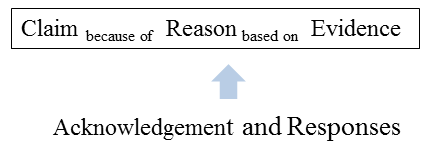
\includegraphics[width=0.60\textwidth]{ClaimReasonEvidence_Ack1}  
  \caption{ClaimReasonEvidenceAcknowledgement}
  \label{fig:Acknowledgement and Response}
\end{center}
\end{figure}
 \end{itemize} 

\chapter{Writing Body Of The Research Paper}
\label{sec:body}
The body of the paper should consist of demonstration of the validity of each
step in the argument. Split parts of the report into chapters and subchapters. Make each chapter coherent: i.e., having a clear beginning and end and a logical connection between the content elements.

\section{Structure Of The Body}
The body of the report consists of the following sections:

\uline{Methods:} "'The methods section of a
research paper provides the information by which a study�s validity is judged.
Therefore, it requires a clear and precise description of how an research was
done, and the rationale for why specific procedures were chosen. The methods section should describe what was
done to answer the research question, describe how it was done, justify the
approach, and explain how the results were analyzed.'" \cite{Kallet2004}.
It must be contain enough information so that the experiment could be
repeated by others to evaluate whether the results are reproducible,
and results and conclusions are valid.
\par \uline{Results:} "'In the Results section,
the results of the experiments, models, or theories should be thoroughly detailed.  
For quantitative research, it is a presentation of the numerical results and data, 
whereas for qualitative research it should be a broader discussion of trends, 
without going into too much detail. For research generating a lot of results,
then it is better to include tables or graphs of the analyzed data and leave 
the raw data in the appendix, so that a researcher can follow up and check your
calculations'"\cite{Day2012}. Rather than displaying isolated and unconnected
charts or figures and findings, a description must be used for linking the results together.

\section{Representation of Visual Evidence}
\label{sec:body:visual_evidence}
"`A claim is assessed by the strength of the
argument supporting it, particularly the soundness of its logic and the quality
of its evidence"'\cite{Booth2003}. But when the data is more complex, a more
systematic presentation is needed to absorb, analyze and understand it.
Readers can get the same data from each of those visually oriented representations, but they will experience different rhetorical effects.
In \cite{Booth2003}, two general guidelines are stated for choosing between tables
and figures:
\begin{itemize}
  \item Choose a table if you want to show very precise numbers and you don't
  want to support your data with a visual image.
  \item Choose a figure if you want to focus on gerneral point rather than
  precise details and you want to emphasize your point using an strong image.
\end{itemize}
\subsection{Constructing tables}
\label{sec:body:visual_evidence:table}
The table of numbers feels precise and objective. It does not impose on us any
predigested outcome. It lets us compare the numbers systematically and come to our own conclusion.
In \cite{Booth2003}, the following principles are suggested for constructing
tables:
\begin{itemize}
  \item Introduce your data with a sentence that explicitly tells the reader
  what to see in them. Then give the table, graph, or chart a title that explicitly names its purpose.
  \item Organize your table in a way that anticipates how your readers will use
  it, and highlight those data most relevant to the claim you want the data to support.
  \item Down the left-hand side of the table, list the items whose
numbers you are presenting to the right.
  \item Across the top, list the categories of data.
  \item Present everything in an order that helps readers find what you want
  them to look for quickly and reliably.
  \item Don�t clutter a table with horizontal and vertical lines separating all
  rows and columns.
\end{itemize}
 It is recommended to avoid vertical lines and double lines. It is a good
 practice to put the units in column heading. The following table serves as a
 guideline for construction of an ideal table:
\begin{table}[h]
\begin{tabular}{@{}llll@{}}
\toprule
Type       & Car                   & Seating Capacity & Price(�)             \\ \midrule
Subcompact & Mini Cooper           & 5                & 19,550               \\
           & Hyundai i10           & 5                & 10,300               \\
           & Ford Fiesta Ka        & 5                & 12,700               \\ \cmidrule(l){4-4} 
           &                       &                  & Avg= 14,183 \\ \midrule
Compact    & BMW 3-Series          & 5                & 28,950               \\
           & VW Golf               & 4                & 17,050               \\
           & Ford Focus            & 5                & 16,850               \\ \cmidrule(l){4-4} 
           &                       &                  & Avg=20,950 \\ \midrule
Full-Size  & BMW 7-Series          & 4                & 74,600               \\
           & Audi A8               & 4                & 69,600               \\
           & Mercedes Benz E-Class & 5                & 71,876               \\ \cmidrule(l){4-4} 
           &                       &                  & Avg=72,025  \\ \midrule
\end{tabular}
\caption{Good Example Table} 
\end{table}

If the above guidelines are not followed, the resulting table can turn into an
ugly table. The following example demonstrates a bad table and conveys the
practices which should be avoided while creating a table.
\begin{table}[h]
\begin{tabular}{|l|l|l|l|}
\hline
Type       & Car                   & Seating Capacity & Price             \\ \hline
Subcompact & Mini Cooper           & 5                & 19,550�              \\\hline 
Subcompact & Hyundai i10           & 5                & 10,300�          \\ \hline 
Subcompact & Ford Fiesta Ka        & 5                & 12,700�               \\\hline 
&                       &                  & Avg= 14,183� \\ \hline
Compact    & BMW 3-Series          & 5                & 28,950�               \\\hline 
Compact    & VW Golf               & 4                & 17,050�               \\\hline 
Compact    & Ford Focus            & 5                & 16,850�               \\\hline 
&                       &                  & Avg=20,950� \\ \hline
Full-Size  & BMW 7-Series          & 4                & 74,600�              \\\hline 
Full-Size  & Audi A8               & 4                & 69,600�          \\\hline 
Full-Size  & Mercedes Benz E-Class & 5                & 71,876�       \\ \hline 
&                       &                  & Avg=72,025� \\ \hline
\end{tabular}
\caption{Bad Example Table} 
\end{table}

\subsection{Constructing Figures}
\label{sec:body:visual_evidence:figure}
As stated in \cite{Edc2010},Figures are crucial in technical communication. They
help readers understand and visualize information that is often hard to understand from text alone. The
word �figures� covers a wide range of items, including photos, sketches,
drawings, graphs, diagrams, flow charts, and maps. 
\par Here are rules for presenting figures clearly and correctly as recommended
in \cite{Edc2010}:
\begin{itemize}
\item \uline{Label the figure.} Give each figure a number and a title that
concisely describe what the label represents.
\item \uline{Indicate the source.} When you include a figure from another
source, include a source line under the figure number and title that indicates 
where the figure was originally published.
\item \uline{Refer to your figure in the text.} Always refer to figures in
the text, explaining their significance and key points. You can�t expect readers to 
focus on the details that impress you about the figure unless you guide 
their view. The reference should precede the figure and identify it by number.
\item \uline{Position the figure effectively.} Place it as close as possible
to its reference in the text. Avoid placing the figure and accompanying text on separate 
pages.
\item \uline{Don�t clutter figures with too many details and labels.}
Include only those details and labels that readers need to understand key points.
\end{itemize}

\subsection{Effective Use Of Graphs}
In \cite{Edc2010},it is stated that Graphs are useful visualize 
data and see relationships. In \cite{Edc2010} it is stated that it is important
to choose the right type of graph to convey your information. Initially the data
must be carefully analyzed to determine the clearest format
for displaying the data. This will help readers to easily grasp the
information. 

In \cite{Turabian2007}, some key guidelines are recommended for designing good
graphs:
\begin{itemize}
  \item Avoid using grid lines. Use grid lines only if  the graphic is complex
  or readers need to see precise numbers.
Make all grid lines light gray,  unless the text will be microfilmed.
  \item Use caution in employing shading or color to convey meaning.  Even if  you print the
paper on a color printer or submit it as a PDF,  it may be printed or copied later on a
black-and-white machine,  and if  it is a dissertation,  it may be microfilmed.  Shading
and color may not reproduce well in any of  these forms.
  \item Never create a three-dimensional chart or graph if  you can represent the same data
in two dimensions.  The added depth contributes nothing and can distort how
readers judge values.
  \item Never use iconic bars (for example,  images of  cars to represent automobile
production).  They add nothing,  can distort how readers judge values,  and look
amateurish.
\end{itemize}

Following example of a graph serves as a guideline for creating graphs:
\begin{figure}[htb]
\begin{center} 
  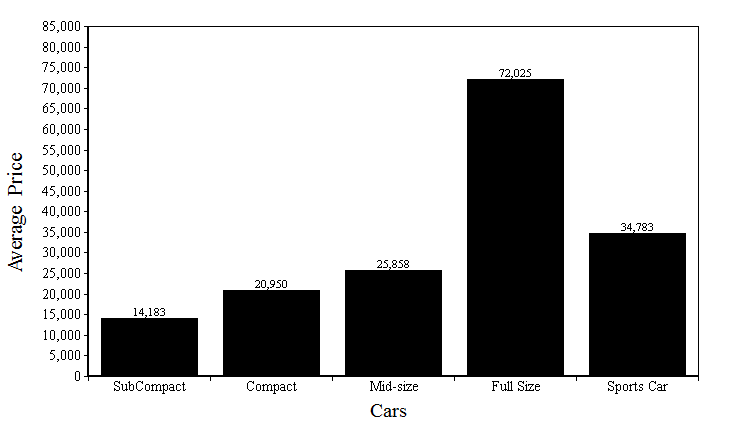
\includegraphics[width=0.60\textwidth]{Graph}  
  \caption{Example Graph}
  \label{fig:example}
\end{center}
\end{figure}


\chapter{Citation Practices}
\label{sec:citation}
As per \cite{Turabian2007}, your first duty as a researcher is to get the facts
right. Your second duty is to state where the facts came from. You must cite the
sources of  the facts,  ideas,  or words that you use in your paper.
\section{Reasons for Citing Sources}
As stated in \cite{Turabian2007}, there are atleast four reasons to cite
sources:
\begin{itemize}
  \item \uline{To give credit.}
  Research is hard work.
Recognition is important for someone who does it, the pride and prestige of 
seeing one�s name associated with knowledge that others value and use. So
when you cite the work of another, you give that writer the recognition he or she has
earned.
\item \uline{To assure about the accuracy of the facts.}
Researchers cite sources to be fair to other researchers but also to earn their
readers�  trust. It is not enough to get the facts right. You must also tell
readers the source of  the facts so that they can judge their reliability,  even check them if they
wish. Readers do not trust a source they don't know and cannot find. If they do
not trust your sources, they will not trust your facts; and if  they do not
trust your facts,  they will not trust your argument.
\item \uline{To show the research tradition that informs your work.}
Researchers cite sources whose data they use, but they also cite work that they
extend,  support, contradict,  or correct.  These citations help readers not only understand 
your specific project but connect it to other research in your field.
\item \uline{To help readers follow or extend your research.}
Many readers use sources cited in a research paper not to check its reliability
but to pursue their own work.  So your citations help others not only to follow 
your footsteps but to strike out in new directions.
\end{itemize}
 
You must never appear to take credit for work that is not your own,  and proper
citation guards against the charge of plagiarism. But it also strengthens your argument
and assists others who want to build on your work.

\section{The Requirements of Citations}
As stated in \cite{Turabian2007}, to fulfill the requirements of  citation, 
you need to know when to include a source citation in your paper and what 
information should be included about the source.

\subsection{Situations Requiring Citations}
As recommended in \cite{Turabian2007}, you should always provide a
citation in the following situations:
\begin{itemize}
  \item When you quote exact words from a source
  \item When you paraphrase ideas that are associated with a specif ic source, 
  even if you don�t quote exact words from it
  \item When you use any idea, data, or method attributable to any source you
  consulted
\end{itemize}

\subsection{Information Required in Citations}
As stated in \cite{Turabian2007}, citation styles differ in the elements
included and in the format of  these elements,  but they have the same aim- to give readers the information they need to identify
and find a source. For most sources, that information must answer these
questions:
\begin{itemize}
  \item Who wrote,  edited,  or translated the text?
  \item What data identify the text? This includes the title and subtitle of  the work; title of  the
	journal,  collection,  or series it appears in, as well as volume number, edition number,
	or other identifying information; and page numbers or other locating information if  the
	reference is to a specif ic part of a larger text.
  \item Who published the text and when? This includes the name of  the publisher and the
place and date of publication or an indication that the document has not been
published.
  \item Where can the text be found? 
\end{itemize}

As per \cite{Turabian2007}, many online sources are like print sources in
everything except medium�for example, an article published in an online journal, online books, newspaper and magazine
articles,  and public documents. Cite an online source of  this type similarly to a print source. 
Other types of  online sources,  such as institutional or personal websites and social
networking services,  are unique to the medium. To cite such a
source,  you will need to give as much information as possible about it in addition to a
URL and access date. It is also a good practice to save these sources so that it
can be reproduced when needed and its existence can be proved if it becomes
unavailable.

\subsection{Preparation of Citations}
As recommended in \cite{Turabian2007}, you can ease the process of preparing and
checking citations if you anticipate what you will need.
\begin{itemize}
  \item Use the most authoritative sources, in their most reliable version
  \item If  a source is available in multiple versions,  always cite the one you actually consulted.
There may be small but important dif ferences between the versions that could af fect
the accuracy of  your quotations or other references to the source.
  \item Record the page number(s) for every quotation and paraphrase.
  \item As you draf t,  clearly indicate every place where you may need to cite a source.  It is
much easier to remove an unnecessary citation when you revise than to remember
where you may have relied on someone else�s ideas.
  \item When your draft is in its final form, ensure that each citation is in
  the correct form, including punctuation and spacing.
\end{itemize}

\section{Citations Management Software}
If  you do the bulk of your bibliographic research online, you may want to consider using
citation management software to collect data about your sources.  Programs like
EndNote, JabRef and Zotero are designed to help you build a �library� of 
citations for a variety of  source types. Later you can plug these citations directly into your paper.
A few things to keep in mind:
\begin{itemize}
  \item Double-check your data.  As you build your library,  check each field against the actual
source as soon as you acquire the data for it.  Make sure that authors�  names,  titles of
works,  dates,  and so forth are accurate and that they are entered in the appropriate
f ields.  You will need to do this whether you entered the data yourself  or exported the
citation f rom a library catalog or other database.
  \item Double-check your citations.  Once they have been inserted in your paper, 
make sure each citation is correctly formatted and punctuated according to the citation style you� ve
chosen. Citation software programs do make errors,  and it remains your
responsibility to ensure that your citations are accurate.
   \item Always keep at least two copies of  your citations library.  If  your school lets you keep a
copy on its server,  make sure you also have a copy on a local drive.
These programs work best for papers that cite only a few types of  the most common
sources.  Articles in academic journals,  especially,  are easy to work with.  If  you cite many
dif ferent types of  sources,  expect to spend extra time correcting your citations library and
editing your f inal paper.  You may choose instead to record the information in the correct
citation format yourself.
\end{itemize}










































































































































































\chapter{Summary and Outlook}

As stated in \cite{Booth2003}, same elements as in Introduction can be used for
conclusion but in reverse order.
\begin{itemize}
\item Start with Your Main Point
State the main point again at the beginning of your conclusion, but state it
more fully. It should not simply repeat the introduction.
\item Add a New Significance or Application
Point to a new significance of the claim which is not mentioned in the
introduction. But care should be taken not to broaden a possible significance 
so much that it seems as the main point. 
\item Add a Call for More Research
More research still to do can be called at the end of the conclusion. That keeps
the conversation alive. Those who pursue your suggestion will review your work, respond to it, and move beyond it.
\end{itemize} 



%%%%%%%%%%%%%%%%%%%%%%%%%%%%%%%%%%%%%%%%%%%%%%%%%%%%%%%%%%%%%%%%%%%%%%%
%% Anhang und Verzeichnisse
%%%%%%%%%%%%%%%%%%%%%%%%%%%%%%%%%%%%%%%%%%%%%%%%%%%%%%%%%%%%%%%%%%%%%%%
\cleardoublepage

\pagenumbering{Roman}
%\begin{appendix}  
%\chapter{Appendix}
   
%\end{appendix}
    
\KOMAoptions{open=any}   
%\addchap{CD-Verzeichnis}
\label{sec:cd}

Dieser Arbeit liegt eine CD bei, \ldots

\markboth{\nomname}{\nomname}
%\nocite{*} 					% alle Quellen auff�hren

%\printnomenclature			% Abk�rzungsverzeichnis
\listoftables				% Tabellenverzeichnis
\listoffigures
%\lstlistoflistings			% Listings-Verzeichnis

\KOMAoptions{open=left}		% war in einem Spezialfall sinnvoll 
\bibliography{Literatur}	% Literaturverzeichnis
\KOMAoptions{open=right}

%\listoftodos				% TODOs, nicht im final Dokument!
%%%%%%%%%%%%%%%%%%%%%%%%%%%%%%%%%%%%%%%%%%%%%%%%%%%%%%%%%%%%%%%%%%%%%%%
      
    
%%%%%%%%%%%%%%%%%%%%%%%%%%%%%%%%%%%%%%%%%%%%%%%%%%%%%%%%%%%%%%%%%%%%%%%
%% Eidesstattliche Erkl�rung
%%%%%%%%%%%%%%%%%%%%%%%%%%%%%%%%%%%%%%%%%%%%%%%%%%%%%%%%%%%%%%%%%%%%%%%
%\chapter*{Eidesstattliche Erkl�rung}
%\thispagestyle{empty}

%\vspace{2cm}

%\noindent Ich, \autor, Matrikel-Nr.\ \matrikelnr, versichere hiermit, dass ich
% meine \arbeitsart\ mit dem Thema
%\begin{quote}
%\textit{\arbeitstitel}
%\end{quote}
%selbst�ndig verfasst und keine anderen als die angegebenen Quellen und
% Hilfsmittel benutzt habe, wobei ich alle w�rtlichen und sinngem��en Zitate als solche gekennzeichnet habe. Die Arbeit wurde bisher keiner anderen Pr�fungsbeh�rde vorgelegt und auch nicht ver�ffentlicht.\\[6ex]

%\ort, den \today\\

%\rule[-0.2cm]{5cm}{0.5pt} 

%\textsc{\autor} 
%%%%%%%%%%%%%%%%%%%%%%%%%%%%%%%%%%%%%%%%%%%%%%%%%%%%%%%%%%%%%%%%%%%%%%%

\end{document}

%%%%%%%%%%%%%%%%%%%%%%%%%%%%%%%%%%%%%%%%%%%%%%%%%%%%%%%%%%%%%%%%%%%%%%%
%% DOKUMENTVORLAGE THOMAS DIETRICH  %%%%%%%%%%%%%%%%%%%%%%%%%%%%%%%%%%%
%%%%%%%%%%%%%%%%%%%%%%%%%%%%%%%%%%%%%%%%%%%%%%%%%%%%%%%%%%%%%%%%%%%%%%%
